\chapter{Mengenal Kecerdasan Buatan dan Scikit-Learn}
Buku umum yang digunakan adalah \cite{russell2016artificial} dan  
untuk sebelum UTS menggunakan buku \textit{Python Artificial Intelligence Projects for Beginners}\cite{eckroth2018python}.
Dengan praktek menggunakan python 3 dan editor anaconda dan library python scikit-learn.
Tujuan pembelajaran pada pertemuan pertama antara lain:
\begin{enumerate}
\item
Mengerti definisi kecerdasan buatan, sejarah kecerdasan buatan, perkembangan dan penggunaan di perusahaan
\item
Memahami cara instalasi dan pemakaian sci-kit learn
\item
Memahami cara penggunaan variabel explorer di spyder
\end{enumerate}
Tugas dengan cara dikumpulkan dengan pull request ke github dengan menggunakan latex pada repo yang dibuat oleh asisten riset.

\section{Teori}
Praktek teori penunjang yang dikerjakan :
\begin{enumerate}
\item
Buat Resume Definisi, Sejarah dan perkembangan Kecerdasan Buatan, dengan bahasa yang mudah dipahami dan dimengerti. Buatan sendiri bebas plagiat[hari ke 1](10)
\item
Buat Resume mengenai definisi supervised learning, klasifikasi, regresi dan unsupervised learning. Data set, training set dan testing set.[hari ke 1](10)
\end{enumerate}

\section{Instalasi}
Membuka https://scikit-learn.org/stable/tutorial/basic/tutorial.html. Dengan menggunakan bahasa yang mudah dimengerti dan bebas plagiat. 
Dan wajib skrinsut dari komputer sendiri.
\begin{enumerate}
\item
Instalasi library scikit dari anaconda, mencoba kompilasi dan uji coba ambil contoh kode dan lihat variabel explorer[hari ke 1](10)
\item
Mencoba Loading an example dataset, menjelaskan maksud dari tulisan tersebut dan mengartikan per baris[hari ke 1](10)
\item
Mencoba Learning and predicting, menjelaskan maksud dari tulisan tersebut dan mengartikan per baris[hari ke 2](10)
\item
mencoba Model persistence, menjelaskan maksud dari tulisan tersebut dan mengartikan per baris[hari ke 2](10)
\item 
Mencoba Conventions, menjelaskan maksud dari tulisan tersebut dan mengartikan per baris[hari ke 2](10)
\end{enumerate}


\section{Penanganan Error}
Dari percobaan yang dilakukan di atas, apabila mendapatkan error maka:

\begin{enumerate}
	\item
	skrinsut error[hari ke 2](10)
	\item
Tuliskan kode eror dan jenis errornya [hari ke 2](10)
	\item
Solusi pemecahan masalah error tersebut[hari ke 2](10)

\end{enumerate}

\section{Andri Fajar S/1164065}
\subsection{sejarah dan perkembangan kecerdasan buatan}
\begin{enumerate}
\item didefinisikan  kecerdasan yang ditunjukkan oleh suatu entitas buatan. Umumnya dianggap komputer. Kecerdasan Buatan (Artificial Intelligence atau AI) didefinisikan sebagai kecerdasan yang ditunjukan oleh suatu entitas buatan. Sistem seperti ini umumnnya dianggao kemputer. Kecerdasan dimasukkan ke dalam mesin (komputer) agar dapat melakukan pekerjaan seperti yang dapat dilakukan manusia. Kecerdasan Buatan (Artificial Intelligence atau AI) didefinikasikan sebagai kecerdasan yang ditinjukkan oleh suatu entitas buatan. Sistem seperti ini umumnya di anggap komputer. Kecerdasan diciptakan dan dimasukkan melakukan pekerjaan seperti yang dapat dilakukan manusia. 
\item Sejarah dan perkembangan kecerdasan buatan terjadi pada musim panas tahun 1956 tercatat adanya seminar mengenai AI di Darmouth College. Seminar pada waktu itu dihadiri oleh sejumlah pakar komputer dan membahas potensi komputer dalam meniru 
kepandaian manusia. Akan tetapi perkembangan yang sering terjadi semenjak diciptakannya LISP, yaitu bahasa kecerdasan buatan yang dibuat tahun 1960 oleh John McCarthy. Istilah pada kecerdasan buatan atau Artificial Intelligence diambil dari Marvin Minsky dari MIT. Dia menulis karya ilmiah berjudul Step towards Artificial Intelligence,The Institute of radio Engineers Proceedings 49, January 1961\cite{ai2011kecerdasani}.
\item Supervised learning merupakan sebuah pendekatan dimana sudah terdapat data yang dilatih, dan terdapat variable yang ditargetkan sehingga tujuan dari pendekatan ini adalah mengkelompokan suatu data ke data yang sudah ada. Sedangkan unsupervised 
learning tidak memiliki data latih, sehingga dari data yang ada, kita mengelompokan data tersebut menjadi 2 bagian atau 3 bagian dan seterusnya.
\item Klasifikasi adalah salah satu topik utama dalam data mining atau machine learning. Klasifikasi yaitu suatu pengelompokan data dimana data yang digunakan tersebut mempunyai kelas label atau target.
\item Regresi adalah Supervised learning tidak hanya mempelajari classifier, tetapi juga mempelajari fungsi yang dapat memprediksi suatu nilai numerik. Contoh, ketika diberi foto seseorang, kita ingin memprediksi umur, tinggi, dan berat orang yang ada pada foto tersebut.
\item Data set adalah cabang aplikasi dari Artificial Intelligence/Kecerdasan Buatan yang fokus pada pengembangan sebuah sistem yang mampu belajar sendiri tanpa harus berulang kali di program oleh manusia.
\item Training set yaitu jika pasangan objek, dan kelas yang menunjuk pada objek tersebut adalah suatu contoh yang telah diberi label akan menghasilkan suatu algoritma pembelajaran.
\subitem Testing set digunakan untuk mengukur sejauh mana classifier berhasil melakukan klasifikasi dengan benar\cite{darujati2012pemanfaatan}.



\end{enumerate}

\subsection{INSTALASI}
Instalasi library scikit dari anaconda, mencoba kompilasi contoh kode dan lihat variable explorer.
\begin {enumerate}
\par
\item Install Aplikasi anaconda
\item buka cmd, lalu install library scikit. ketikan perintah conda install scikit-learn 
\par
\begin{figure}[ht]
\centering
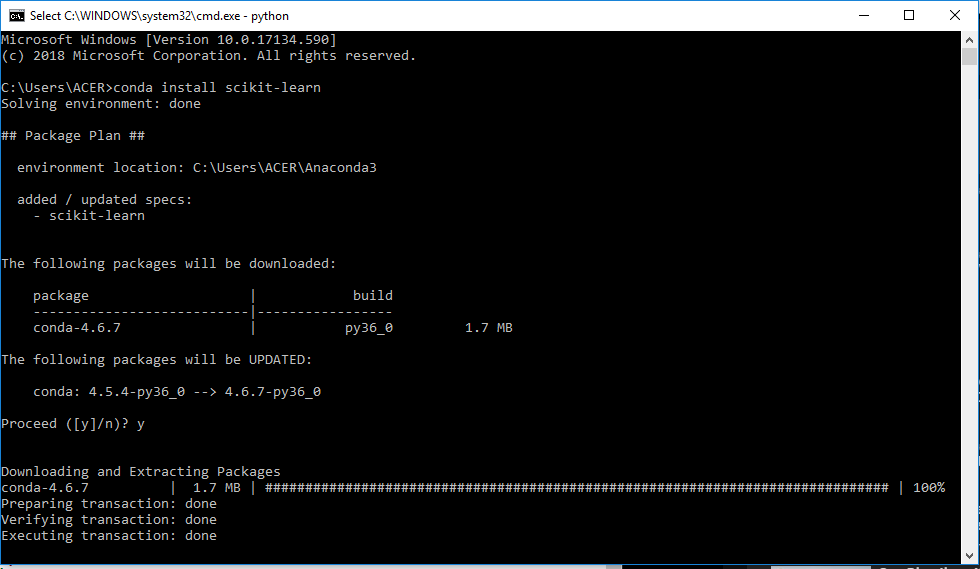
\includegraphics[scale=0.5]{figures/111.png}
\caption{Install library scikit}
\label{contoh1}
\end{figure}
\par

\item cek version anaconda dan python
\par
\begin{figure}[ht]
\centering
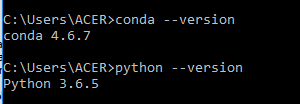
\includegraphics[scale=0.7]{figures/222.png}
\caption{version anaconda dan python}
\label{contoh2}
\end{figure}
\par

\item update library scikit dengan perintah pip install -U scikit-learn
\par
\begin{figure}[ht]
\centering
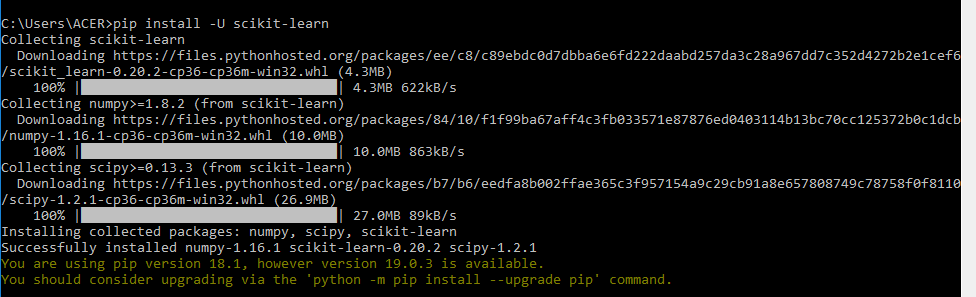
\includegraphics[scale=0.5]{figures/333.png}
\caption{update library scikit}
\label{contoh3}
\end{figure}
\par

\item test compile
\par
\begin{figure}[ht]
\centering
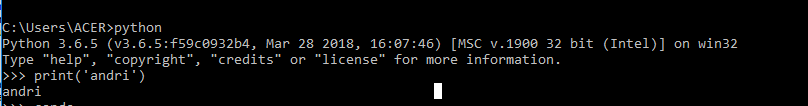
\includegraphics[scale=0.5]{figures/444.png}
\caption{test compile}
\label{contoh4}
\end{figure}
\end {enumerate}
\par

Mencoba Loading an example dataset
\begin {enumerate}
\par
\item Dari skalearn menginport dataset kemudian dataset nge load dari iris dan digits
\par
\begin{figure}[ht]
\centering
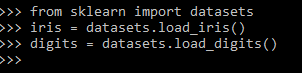
\includegraphics[scale=0.5]{figures/555.png}
\caption{import dataset}
\label{contoh5}
\end{figure}
\par
\item mencoba menampilkan data digits
\par
\begin{figure}[ht]
\centering
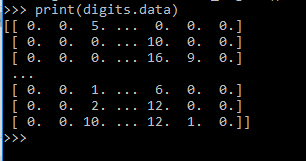
\includegraphics[scale=0.5]{figures/666.png}
\caption{data digits}
\label{contoh6}
\end{figure}
\end {enumerate}

